
% \PID На је дат сигнал $x[n]$ чија је $\mathcal{Z}$-трансформација позната као $X(z)$. Амплитудски 
% спектар тог сигнала приказан је на слици \ref{\ID.um.jw}. Сигнал $y[n]$ добија се уметањем по 
% две нуле између свака два одбирка сигнала $x[n]$ као што је приказано на слици \ref{\ID.um.x}.
% %
% \begin{figure}[ht!]
%     \centering
%     \begin{subfigure}{0.49\textwidth}
%         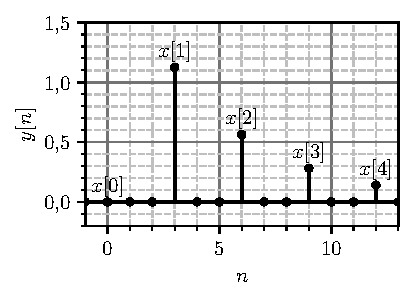
\includegraphics{fig/umetanje_def.pdf}
%         \caption{N}
%         \label{\ID.um.x}    
%     \end{subfigure}
%     %
%     \begin{subfigure}{0.49\textwidth}
%         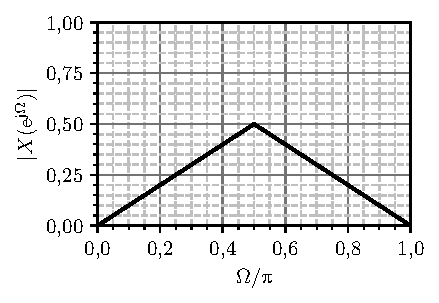
\includegraphics{fig/umetanje_x_jw.pdf}
%         \caption{}
%         \label{\ID.um.jw}    
%     \end{subfigure}
%     \caption{Уз задатак.}
% \end{figure}
